% =================================================================
% 第2章 三维高斯溅射与几何先验理论基础
% =================================================================
\chapter{三维高斯溅射与几何先验理论基础}
\label{chap:theory_foundation}

本章旨在为后续面向工业场景的三维高斯溅射（3D Gaussian Splatting, 3DGS）改进算法研究奠定理论基础与技术背景。
围绕工业数字孪生的实际应用需求，本文首先讨论工业场景对于高保真、实时三维表征能力的现实要求，并结合弱纹理、高反光等典型复杂环境，分析传统三维重建方法在此类场景下所面临的适应性不足与性能瓶颈。
在此基础上，对新视角合成技术的发展过程进行梳理，重点比较神经辐射场（NeRF）与三维高斯溅射在表示方式、渲染机制及计算特征等方面的本质差异。
进一步地，本章将对 3DGS 的核心数学原理展开分析，内容包括三维高斯的显式参数化表示、投影变换过程，以及依托可微光栅化实现的自适应密度控制优化机制。
结合本文的研究目标，还将讨论在显式辐射场框架中引入多模态几何先验（如深度信息）的理论依据及其必要性，从而为后续章节的方法设计与算法创新提供支撑。

\section{工业数字孪生与三维重建技术}
\label{sec:digital_twin_reconstruction}

随着智能制造与工业 4.0 的深入推进，工业数字孪生（Industrial Digital Twin）作为连接物理实体与虚拟空间的桥梁，正在成为实现工业数字化转型的关键技术。
在数字孪生系统中，物理世界中的设备、产线及工厂环境需要在虚拟空间中进行高精度的几何建模与外观还原，即实现“虚实映射”。这一过程高度依赖于底层的高效、高精度三维重建技术。

\subsection{工业数字孪生的概念与三维表征需求}
\label{subsec:dt_concept_needs}

工业数字孪生是指通过集成多源传感器数据、历史运行数据以及物理模型，在虚拟空间中构建与物理实体在形态、状态及行为上高度一致的动态副本。
在诸如智能制造产线监控、大型设备远程巡检、以及虚拟现实（VR）辅助装配等典型工业应用中，数字孪生系统不仅需要实时反映物理设备的运行状态，更需要提供具备极高沉浸感和真实感的视觉呈现。

具体而言，工业场景对三维表征技术提出了以下几项极为严苛的需求：
第一，\textbf{高保真度的几何与外观还原}。
工业设备通常包含复杂的机械结构（如齿轮、细小管道、线缆）以及多样的材质属性（如金属加工件的镜面反射、涂装表面的漫反射）。
三维表征技术必须能够精确刻画这些高频细节，避免在虚拟漫游时出现严重的结构伪影或材质失真。
第二，\textbf{实时渲染与交互能力}。
工业数字孪生系统通常需要接入海量的实时物联网（IoT）数据，并支持操作人员在复杂的三维场景中进行流畅的视点切换与漫游。
这就要求底层渲染引擎必须具备高帧率（通常要求达到 30 FPS 或 60 FPS 以上）的实时渲染能力，传统的基于庞大面片数量的网格模型（Mesh）或计算复杂度极高的隐式神经表示往往难以满足这一实时性约束。
第三，\textbf{鲁棒的复杂环境适应性}。
工业现场环境恶劣，光照条件复杂且多变（如车间内的局部强光源、阴影交错），且设备表面往往存在大面积的无纹理区域（如纯色机床外壳）或高反光金属材质。
如何在这些极端观测条件下获取稳定、准确的三维表征，是工业数字孪生面临的重大挑战。

\begin{figure}[htbp]
    \centering
    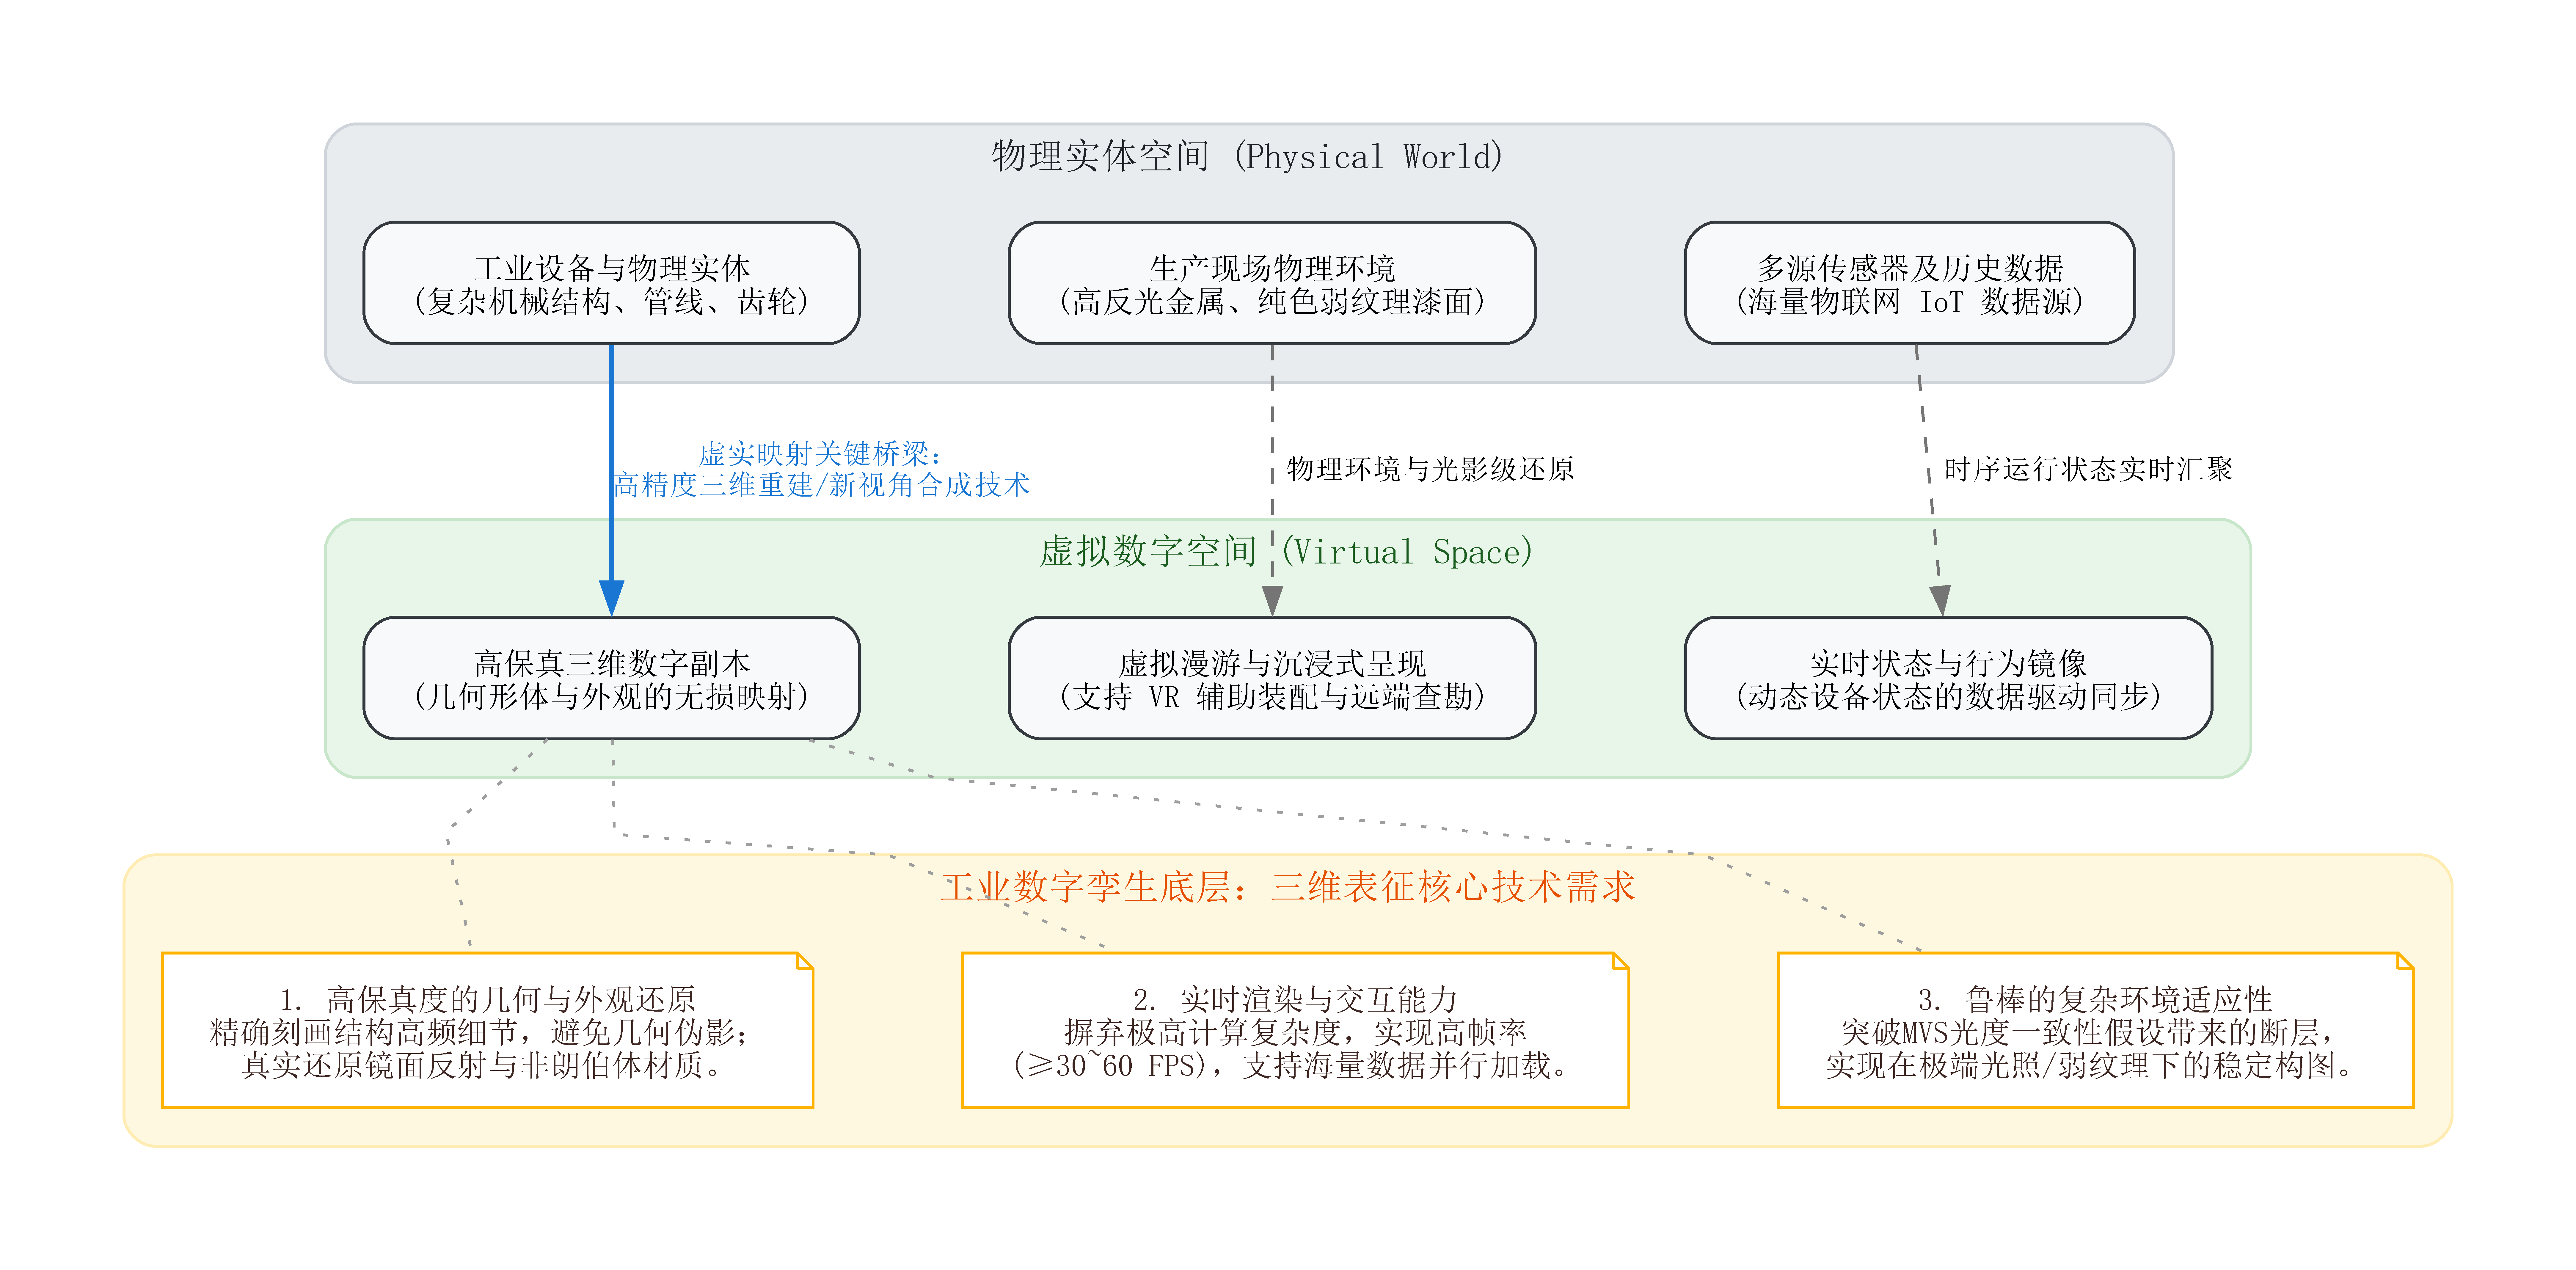
\includegraphics[width=0.95\linewidth]{figures/chap2/fig_2_1_Architecture_StraightLines.pdf}
    \caption{工业数字孪生系统中的虚实映射架构及三维表征需求}
    \label{fig:industrial_dt_architecture}
\end{figure}

\subsection{传统三维重建技术及其在工业场景的局限性}
\label{subsec:traditional_reconstruction}

在三维高斯溅射及神经辐射场等新视角合成技术兴起之前，工业领域的三维模型获取主要依赖于计算机辅助设计（CAD）建模与传统基于多视图几何（Multiple View Geometry）的三维重建技术。
CAD 建模虽然精度极高，但主要用于产品设计阶段，难以反映设备在实际运行环境中的真实磨损、形变及光照状态，且人工建模成本高昂，无法实现场景的快速自动化构建。

传统基于多视图几何的三维重建管线通常包含运动恢复结构（Structure from Motion, SfM）\cite{schonberger2016structure} 和多视图立体视觉（Multi-View Stereo, MVS）\cite{furukawa2015multi} 两个核心阶段。
SfM 算法首先通过提取图像间的二维特征点（如 SIFT、SURF 等），并进行特征匹配与极线几何约束，联合估计出相机的内外参数以及稀疏的场景点云。
随后，MVS 算法利用已知的相机位姿，通过计算深度图或进行密集的光度一致性匹配，生成稠密的三维点云，最终通过泊松表面重建（Poisson Surface Reconstruction）等算法提取出网格模型。

然而，将其直接应用于工业场景时，传统 MVS 算法暴露出显著的局限性：
首先，\textbf{对弱纹理和高反光材质极其敏感}。
MVS 算法的核心在于跨视角的特征匹配与光度一致性假设（即假设同一个物理点在不同视角下的颜色保持不变）。
但在工业车间中，大量的金属设备表面具有强烈的镜面反射（Specular Highlight），其观测颜色会随视角的改变而剧烈变化，直接打破了光度一致性假设。同时，设备外壳等大面积纯色区域缺乏可供提取的局部特征，导致 SfM 阶段特征匹配失败，MVS 阶段无法计算准确的深度值。
这最终体现为重建出的点云在金属表面和弱纹理区域出现大面积的空洞、断层或严重的离群噪声。
其次，\textbf{复杂拓扑结构的重建能力不足}。
工业现场的线缆、防护网等细小结构在二维图像中所占像素极少，传统算法在进行深度图融合与网格提取时，容易将这些高频结构作为噪声过滤掉，或者发生错误的几何粘连。
最后，\textbf{离散化表示带来的渲染限制}。
传统管线最终输出的点云或网格模型是固定的离散几何结构，在渲染时难以自然地表达半透明材质或复杂的体积光散射效应，且在近距离观察时容易出现明显的锯齿和面片感，无法达到照片级（Photorealistic）的渲染质量。

综上所述，传统三维重建技术在面临工业复杂环境时，难以兼顾几何结构的完整性与视觉呈现的高保真度。
这一现状迫切需要引入一种能够突破传统光度一致性限制、具备强大学习与表征能力的新型三维场景建模方法。

% =================================================================
% 第2章 2.2节 辐射场与新视角合成技术演进
% =================================================================

\section{辐射场与新视角合成技术演进}
\label{sec:nvs_evolution}

在上一节探讨了传统多视图几何（MVS）在工业场景中的局限性后，本节将视线转向近年来引领三维视觉变革的新视角合成（Novel View Synthesis, NVS）技术。
新视角合成旨在给定一组场景的稀疏视角图像及对应的相机位姿参数后，合成该场景在任意未见视角下的逼真图像 。
在 3D Gaussian Splatting (3DGS) 出现之前，该领域经历了从显式离散几何（如点云、网格、体素）到隐式神经表示（Implicit Neural Representation），再向新型连续-离散混合显式表征（如 3DGS）的重大范式演进。
本节将深入剖析神经辐射场（NeRF）的基础数学原理，并系统论证其在工业数字孪生应用中所面临的技术瓶颈。

\subsection{基于隐式神经表示的新视角合成基础}
\label{subsec:nerf_basics}

神经辐射场（Neural Radiance Fields, NeRF）的提出标志着三维场景表征进入了“隐式计算”时代。
NeRF 摒弃了传统的离散几何载体，转而通过一个多层感知机（Multilayer Perceptron, MLP）网络，将连续的三维空间隐式地参数化 。

具体而言，NeRF 将场景建模为一个连续的五维函数。
网络的输入为空间三维坐标 $\bm{x} = (x, y, z)$ 和观测视角方向 $\bm{d} = (\theta, \phi)$，输出为该空间点的体积密度（Volume Density）$\sigma$ 和与视角相关的辐射颜色（Color）$\bm{c} = (r, g, b)$ 。这一映射关系可抽象为：
\begin{equation}
    F_{\Theta}: (\bm{x}, \bm{d}) \to (\bm{c}, \sigma)
\end{equation}
其中，$\Theta$ 为 MLP 网络的权重参数。
为了保证场景几何的一致性，密度 $\sigma$ 仅由空间位置 $\bm{x}$ 决定，而颜色 $\bm{c}$ 则同时依赖于位置 $\bm{x}$ 和视角 $\bm{d}$，从而使得模型能够拟合出镜面反射等复杂的非朗伯体（Non-Lambertian）效应。

在获取了空间点属性后，NeRF 采用经典的体积渲染方程（Volume Rendering Equation）来合成二维图像 。给定空间中任意一条由相机光心发出、穿过图像像素的射线 $\bm{r}(t) = \bm{o} + t\bm{d}$（$\bm{o}$ 为相机原点，$t$ 为沿射线的步长），该射线对应的像素颜色 $C(\bm{r})$ 通过对射线路径上的连续点进行积分计算得出 ：
\begin{equation}
    C(\bm{r}) = \int_{t_n}^{t_f} T(t) \sigma(\bm{r}(t)) \bm{c}(\bm{r}(t), \bm{d}) dt
\end{equation}
在此公式中，$t_n$ 和 $t_f$ 分别代表射线的近端与远端物理边界；
$\sigma(\bm{r}(t))$ 为空间点的位置密度，反映了光线在该点被阻挡的概率；
$\bm{c}(\bm{r}(t), \bm{d})$ 为依赖于视角的发射颜色 。
$T(t)$ 被称为累积透射率（Accumulated Transmittance），其物理意义为射线从 $t_n$ 传播到当前深度 $t$ 且未被任何粒子遮挡或吸收的概率 ，其严格的积分定义为：
\begin{equation}
    T(t) = \exp\left(-\int_{t_n}^{t} \sigma(\bm{r}(s)) ds\right)
\end{equation}

在实际的工程实现中，由于计算机无法进行连续积分，NeRF 采用了离散化的分层体积采样（Hierarchical Volume Sampling）策略。
将射线划分为 $N$ 个均匀的区间，并在每个区间内进行随机均匀采样。离散化后的体积渲染方程近似为：
\begin{equation}
    \hat{C}(\bm{r}) = \sum_{i=1}^{N} T_i (1 - \exp(-\sigma_i \delta_i)) \bm{c}_i
\end{equation}
其中，$\delta_i = t_{i+1} - t_i$ 为相邻采样点之间的距离，$T_i = \exp(-\sum_{j=1}^{i-1} \sigma_j \delta_j)$ 为离散透射率。

此外，为了使由低频偏置（Low-frequency Bias）主导的 MLP 能够学习到工业场景中复杂的高频几何纹理，NeRF 引入了高频位置编码（Positional Encoding, PE）机制。
通过一组正弦和余弦函数，将低维的输入坐标映射到高维特征空间：
\begin{equation}
    \gamma(p) = \left( \sin(2^0 \pi p), \cos(2^0 \pi p), \dots, \sin(2^{L-1} \pi p), \cos(2^{L-1} \pi p) \right)
\end{equation}
其中，$L$ 控制着编码的最高频段。这一机制极大地提升了隐式场对尖锐边缘和精细纹理的表征能力。

\subsection{隐式神经辐射场在工业场景中的应用瓶颈}
\label{subsec:nerf_bottlenecks}

尽管 NeRF 及其变体（如 Mip-NeRF, Instant-NGP）在新视角合成质量上取得了革命性的突破，但将其直接部署于工业数字孪生系统时，仍暴露出几项难以调和的技术瓶颈。
这些瓶颈不仅阻碍了其在实际工程中的落地，也正是促使学术界转向探寻诸如 3DGS 等新型显式表征的核心驱动力。

\textbf{第一，极高的计算复杂度与实时渲染的鸿沟。}
工业数字孪生（如虚拟产线漫游、设备远程监控）对渲染引擎的帧率有着严苛的下限要求（通常 $\ge 30$ FPS）。
然而，NeRF 的渲染过程高度依赖于密集的光线步进（Ray Marching）采样 。
为了渲染一张 $1920 \times 1080$ 分辨率的高清图像，需要发射约 200 万条射线，若每条射线采样 128 个点，则单帧渲染需执行超过 2.5 亿次的 MLP 网络前向推理 。
这种极度密集的计算负荷导致原始 NeRF 的渲染速度通常仅为秒级甚至分钟级每帧，完全无法满足工业级实时交互的需求。
即便后续的加速方案（如预计算网格、哈希编码）在一定程度上缓解了推理压力，但依然难以在消费级硬件上兼顾超高分辨率与高帧率 。

\textbf{第二，高频几何提取困难与拓扑结构失真。}
在工业制造与检测场景中，数字孪生系统不仅需要“看起来真实”（高保真渲染），更需要“用起来准确”（高精度几何）。
工程师往往需要从三维场中提取出具有明确物理边界的网格（Mesh）进行碰撞检测或应力分析。
然而，NeRF 的核心本质是一个连续的“密度云”（Density Field），缺乏显式的表面边界。
当使用移动立方体算法（Marching Cubes）从密度场中提取等值面（Iso-surface）时，极易在物体边缘产生噪声、坑洼，甚至出现悬浮于空中的“伪影”（Floaters）。
特别是在面对管线密集、拓扑结构复杂的工业设备时，隐式表征往往会将本该独立的细小部件粘连在一起，破坏了工业模型的严谨拓扑关系。

\textbf{第三，对金属高反光与弱纹理材质的病态拟合。}
这是限制纯视觉三维重建技术在工业场景应用的最大痛点。
工业厂房内广泛存在大面积纯色漆面的机箱外壳（弱纹理）以及抛光金属加工件（高反光）。
NeRF 在试图拟合这些区域时，由于缺乏足够的高频图像梯度约束，其 MLP 往往会利用“颜色参数（依赖于视角）”来强行掩盖“几何参数（密度场）”的错误。
具体表现为：网络在金属表面前方凭空生成一层半透明的“雾状伪影”来模拟反光效果，导致该处的真实几何表面发生严重的向内坍塌或向外膨胀。
这种“以几何换光影”的病态优化，使得隐式场在复杂材质下的三维结构变得极不可靠。

\subsection{从隐式到显式：三维表征技术的范式转变}
\label{subsec:paradigm_shift}

鉴于隐式神经表示在计算效率与显式几何约束上存在的先天不足，三维视觉研究范式开始发生转变：逐渐摒弃耗时的 MLP 射线查询，回归到对计算机图形学管线（Graphics Pipeline）更加友好的\textbf{显式或连续-离散混合表征}。

研究者们试图利用体素网格（Voxel Grids）、点云（Point Clouds）或多分辨率哈希表来存储场景特征。
在这一演进路线的顶端，\textbf{三维高斯溅射（3D Gaussian Splatting, 3DGS）}脱颖而出。
不同于 NeRF 使用的隐式神经网络，3DGS 创造性地利用数百万个离散的、可微分优化的各向异性三维高斯球来拟合场景 。
它彻底抛弃了低效的体积光线步进，转而结合高效的可微光栅化（Differentiable Rasterization）技术，在保留甚至超越 NeRF 照片级渲染质量的同时，直接通过 GPU 并行管线实现了高达百帧以上的实时渲染 。

为了直观地展示各类三维场景表征技术在工业数字孪生应用背景下的优劣，表 \ref{tab:representation_comparison} 进行了系统的多维对比。

\begin{table}[htbp]
    \centering
    \caption{三维场景表征技术对比及工业应用适配度分析}
    \label{tab:representation_comparison}
    \renewcommand{\arraystretch}{1.3} % 增加行高使表格更美观
    \begin{tabular}{l c c c c c}
        \toprule
        \textbf{表征方法} & \textbf{数据结构} & \textbf{渲染速度} & \textbf{优化/训练时间} & \textbf{几何表面提取} & \textbf{高频材质表现力} \\
        \midrule
        传统多视图网格 (MVS) & 显式离散 & 极快 (直接光栅化) & 中等 (数小时) & 清晰、直接 & 差 (固化纹理, 无视点相关) \\
        神经辐射场 (NeRF) & 隐式连续 & 极慢 (秒/帧) & 极慢 (十余小时) & 困难 (易含噪声) & 强 (隐式拟合能力极强) \\
        加速隐式场 (Instant-NGP) & 混合 (哈希+MLP) & 较快 (实时) & 快 (数分钟) & 困难 & 较强 \\
        \textbf{三维高斯溅射 (3DGS)} & \textbf{显式混合} & \textbf{极快 (100+ FPS)} & \textbf{快 (数十分钟)} & \textbf{较易 (可提点云)} & \textbf{极强 (各向异性表达)} \\
        \bottomrule
    \end{tabular}
\end{table}

综上所述，3DGS 以其显式的结构优势、极致的渲染性能以及对高频细节的优秀拟合能力，成为了当下工业数字孪生底层重建的最优解。
然而，正由于其采用了显式的空间离散点云（高斯球）结构，在面对工业场景特有的弱纹理与镜面反射时，依然存在高斯球空间位置发散的问题，这就需要我们进一步深入剖析 3DGS 的核心数学原理，并探讨引入深度等几何先验的必要性。
这也将是本章后续小节展开论述的核心内容。


% =================================================================
% 第2章 2.3节 三维高斯溅射核心原理与多模态几何先验
% =================================================================

\section{三维高斯溅射核心数学原理与多模态几何先验}
\label{sec:3dgs_core_principles}

如前文所述，在工业场景的复杂材质与极端光照条件下，传统的隐式神经表征面临着渲染效率低、几何提取难等瓶颈。三维高斯溅射（3D Gaussian Splatting, 3DGS）\cite{kerbl20233d} 作为一种革命性的显式辐射场表征方法，通过将场景参数化为数百万个具有各向异性（Anisotropic）的三维高斯椭球体，并结合可微分光栅化器，实现了兼顾极高保真度与实时帧率的新视角合成。
然而，3DGS 极度依赖初始点云的质量，本节将在深入剖析 3DGS 核心数学原理的基础上，探讨引入多模态感知（如 LiDAR）进行几何先验约束与空间坐标对齐的必要性。

\subsection{三维高斯的显式参数化表示}
\label{subsec:gaussian_representation}

在 3DGS 的理论框架中，连续的三维场景被离散化为一组空间中的三维高斯函数。
每一个三维高斯体 $G(\bm{x})$ 均由其在三维空间中的均值（即中心位置）$\bm{\mu} \in \mathbb{R}^3$ 和三维协方差矩阵（Covariance Matrix）$\bm{\Sigma} \in \mathbb{R}^{3 \times 3}$ 唯一确定，其标准的多元高斯概率密度函数可表示为：
\begin{equation}
    G(\bm{x}) = \exp \left( -\frac{1}{2} (\bm{x} - \bm{\mu})^T \bm{\Sigma}^{-1} (\bm{x} - \bm{\mu}) \right)
\end{equation}

为了确保在基于梯度的优化过程中协方差矩阵 $\bm{\Sigma}$ 始终保持半正定（Positive Semi-Definite）的物理属性，3DGS 巧妙地将其分解为一个缩放矩阵（Scaling Matrix）$\bm{S}$ 和一个旋转矩阵（Rotation Matrix）$\bm{R}$：
\begin{equation}
    \bm{\Sigma} = \bm{R} \bm{S} \bm{S}^T \bm{R}^T
\end{equation}
其中，缩放矩阵 $\bm{S} = \text{diag}(s_x, s_y, s_z)$ 由三个独立的一维缩放因子构成，控制着高斯体在三个主轴方向上的尺寸，赋予了其各向异性的表达能力；旋转矩阵 $\bm{R}$ 则由一个单位四元数（Quaternion）$\bm{q} = (q_r, q_i, q_j, q_k)$ 映射而来，使得旋转操作在优化过程中连续且可导，避免了欧拉角带来的万向节死锁（Gimbal Lock）问题。

除了几何属性外，为了进行渲染，每个三维高斯体还绑定了两个关键的外观属性：不透明度（Opacity）$\alpha \in [0,1]$（通过 Sigmoid 函数将实数域映射至有效区间），以及用于表示视角相关颜色的球谐函数（Spherical Harmonics, SH）系数 $\bm{C}$。
相较于 NeRF 庞大的 MLP，这种显式的参数化集合 $\mathcal{P} = \{\bm{\mu}_i, \bm{S}_i, \bm{q}_i, \alpha_i, \bm{C}_i\}_{i=1}^{N}$ 极大地降低了场景存储的计算冗余。

\subsection{基于可微分光栅化的投影与渲染管线}
\label{subsec:differentiable_rasterization}

在获取了三维高斯的参数后，新视角合成的核心步骤是将其投影至二维图像平面。
这一过程借鉴了计算机图形学中的经典溅射（Splatting）技术 \cite{zwicker2001surface}。
给定相机的观察变换矩阵（Viewing Transformation）$\bm{W}$，三维空间中的协方差矩阵 $\bm{\Sigma}$ 投影至二维相平面上的协方差矩阵 $\bm{\Sigma}'$ 的近似计算公式为：
\begin{equation}
    \bm{\Sigma}' = \bm{J} \bm{W} \bm{\Sigma} \bm{W}^T \bm{J}^T
\end{equation}
在此公式中，$\bm{J}$ 为射影变换的仿射近似雅可比矩阵（Jacobian of the affine approximation of projective transformation）。
由于仅保留了 $\bm{\Sigma}'$ 左上角的 $2 \times 2$ 子矩阵，该操作有效地将三维椭球体“压扁”为二维图像平面上的椭圆。

在渲染阶段，3DGS 抛弃了 NeRF 耗时的光线步进采样，采用了一种基于图块（Tile-based）的高效可微光栅化架构。
图像平面被划分为 $16 \times 16$ 像素的连续图块（Tiles），算法根据每个三维高斯投影后的二维包围盒（Bounding Box），
计算其与各个图块的相交情况。随后，对每个图块内的高斯体根据其中心深度（即距相机光心的距离）进行严格的前向-后向排序（Front-to-back Sorting）。

最终，对于图像平面上的任意像素 $\bm{p}$，其渲染颜色 $C(\bm{p})$ 通过经典的 $\alpha$-blending（阿尔法混合）公式，沿着深度顺序对覆盖该像素的 $\mathcal{N}$ 个高斯体进行累加求和：
\begin{equation}
    C(\bm{p}) = \sum_{i=1}^{\mathcal{N}} c_i \alpha_i' \prod_{j=1}^{i-1} (1 - \alpha_j')
\end{equation}
其中，$c_i$ 是通过当前视角方向结合球谐系数评估出的颜色，
$\alpha_i'$ 是考虑了高斯空间衰减后的二维投影不透明度：$\alpha_i' = \alpha_i \times \exp(-\frac{1}{2}\Delta\bm{p}^T \bm{\Sigma}'^{-1} \Delta\bm{p})$。
该管线不仅实现了 GPU 级别的极高并行渲染度，且由于每一步操作均可完全可导（Fully Differentiable），使得反向传播优化成为可能。

\subsection{自适应密度控制与优化缺陷}
\label{subsec:adaptive_density_control}

3DGS 场景表征的精细化依赖于对高斯集合的迭代优化与自适应密度控制（Adaptive Density Control）。
在训练期间，算法利用渲染图像与真实视角的 Ground Truth 图像之间的 $L_1$ 损失与 D-SSIM（结构相似性）损失，通过随机梯度下降（SGD）计算上述所有参数的梯度。

更为关键的是，3DGS 设计了一套启发式的拓扑结构演化机制，周期性地对场景中的高斯体进行“克隆（Clone）”、“分裂（Split）”和“裁剪（Prune）”：
\begin{itemize}
    \item \textbf{克隆（Clone）：} 对于试图拟合高频细节但体积较小的“欠重建”（Under-reconstructed）区域，系统会复制该高斯体并沿着位置梯度方向移动，增加局部密度。
    \item \textbf{分裂（Split）：} 对于覆盖了较大空间范围或跨越了复杂几何边界的“过度重建”（Over-reconstructed）高斯体，系统将其分裂为两个体积更小的高斯体，并通过缩放因子降低其覆盖范围。
    \item \textbf{裁剪（Prune）：} 周期性地剔除不透明度 $\alpha$ 低于设定阈值（如 $\epsilon = 0.005$）的透明高斯体，以及在世界空间中体积过度膨胀的高斯体，以控制显存占用并减少渲染伪影。
\end{itemize}

\textbf{工业场景中的优化崩溃：}
然而，这套自适应生长机制在工业场景中存在致命缺陷。
3DGS 的初始高斯球位置极度依赖于传统 SfM（如 COLMAP）输出的稀疏点云。
正如 2.1 节所述，工业设备大面积的无纹理外壳与反光金属导致 SfM 提取的点云极度稀疏甚至在这些区域出现大面积空白。
当初始点云缺失时，3DGS 无法在正确的位置“播种”初始高斯体。
在后续的优化中，为了降低图像域的损失，算法会迫使远处的高斯体发生病态的极端“膨胀”或在空中错误地“克隆”伪影，导致原本平滑的工业设备表面呈现出严重的“絮状”或“刺状”几何失真。
这也深刻揭示了在显式辐射场中引入外部准确的几何约束（Geometric Priors）作为初始化骨架的迫切需求。

\subsection{多模态感知引入与空间位姿解算}
\label{subsec:multimodal_pose_alignment}

针对传统纯视觉重建算法（SfM）在弱纹理区域极易出现的特征匹配失败与点云稀疏坍塌问题，
引入多模态传感器（尤其是激光雷达 LiDAR 及高精度 IMU）成为了打破几何约束瓶颈的核心方案。

LiDAR 的工业应用优势在于其属于主动发光传感器，通过发射红外激光脉冲测量飞行时间（Time of Flight, ToF）来获取深度信息。
因此，它对环境光照变化完全免疫，且不受工业场景中大面积无纹理区域（如白墙、光滑金属外壳）的干扰。
LiDAR 扫描生成的稠密点云（Point Cloud, 通常以 .ply 或 .pcd 格式存储）能够直接为 3DGS 提供具备绝对真实物理尺度的初始稠密几何骨架。

在此新视角合成管线中，精确的相机外参（Camera Extrinsics）是保证辐射场收敛的前提。
借助 LiDAR 内部集成的同步定位与建图（SLAM）算法及惯性测量单元，扫描设备能够直接输出高精度、无尺度漂移的传感器运动轨迹（Trajectory）。
然而，直接利用该硬件轨迹驱动 3DGS 渲染需要跨越复杂的坐标系映射障碍。

我们定义激光雷达局部坐标系为 $\mathcal{F}_{L}$，高分辨率 RGB 相机坐标系为 $\mathcal{F}_{C}$。
空间中任意物理点 $\bm{P}$ 在这两个异构传感器坐标系下的齐次坐标系转换关系，可通过严格的刚体变换（Rigid Transformation）模型进行描述：
\begin{equation}
    \bm{P}_C = \bm{T}_{L \to C} \bm{P}_L = 
    \begin{bmatrix} 
    \bm{R}_{ext} & \bm{t}_{ext} \\ 
    \bm{0}^T & 1 
    \end{bmatrix} 
    \bm{P}_L
\end{equation}
其中，$\bm{T}_{L \to C} \in SE(3)$ 是多模态系统的外参校准矩阵。
$\bm{R}_{ext} \in SO(3)$ 为 $3 \times 3$ 的正交旋转矩阵，表征激光雷达坐标轴与相机坐标轴在空间中的相对角度偏转；
$\bm{t}_{ext} \in \mathbb{R}^3$ 为平移向量，代表两个传感器光学中心在三维空间中的物理安装偏差。

通过精确的标定板（Calibration Target）或在线互信息配准算法获取 $\bm{T}_{L \to C}$ 后，
我们可以将 LiDAR 获取的绝对尺度稠密点云无缝投影至相机坐标系，从而完美替代 COLMAP 脆弱的 SfM 初始化结果。
这种基于多模态感知的几何先验注入，不仅为 3DGS 提供了极高置信度的空间初始均值 $\bm{\mu}_i$，
更从根本上规避了自适应密度控制在弱纹理区域因缺乏初始锚点而引发的几何崩溃，为实现工业数字孪生的高精度虚实映射扫清了底层障碍。

% 预留图表位
\begin{figure}[htbp]
    \centering
    % \includegraphics[width=0.9\textwidth]{figures/3dgs_pipeline_with_lidar.pdf}
    \caption{结合多模态空间位姿对齐的 3D Gaussian Splatting 渲染与优化管线}
    \label{fig:3dgs_pipeline}
\end{figure}



% =================================================================
% 第2章 2.4节 本章小结
% =================================================================

\section{本章小结}
\label{sec:chap2_summary}

本章立足于工业数字孪生对高保真、实时三维渲染的迫切需求，系统性地梳理了三维场景重建与新视角合成技术的理论基础及其演进脉络。
首先，分析了传统基于多视图几何（SfM/MVS）的三维重建技术在面对工业现场常见的高反光金属部件与大面积弱纹理设备时，存在的特征匹配失效与点云严重缺失问题。
其次，深入对比了隐式神经辐射场（NeRF）与新型显式表征三维高斯溅射（3DGS）的技术差异，
指出 3DGS 虽然通过引入各向异性三维高斯球与基于图块的可微光栅化管线，成功突破了工业级实时渲染与高频几何细节还原的计算瓶颈，
但其启发式的自适应密度控制机制在复杂场景下极易陷入局部最优，且高度依赖于高质量的初始点云骨架。

针对上述理论缺陷，本章详细剖析了 3DGS 的核心数学表达与优化管线，并着重论证了在显式辐射场中引入多模态感知数据（如 LiDAR 稠密点云）的必要性。
通过严谨的空间位姿解算与刚体变换矩阵对齐，外部高精度几何先验的注入能够从根本上替代脆弱的纯视觉初始化，规避高斯球在弱纹理区域发生的病态膨胀与絮状几何失真。

总体而言，本章的理论推导与局限性分析，深刻揭示了 3DGS 在实现工业级虚实映射过程中面临的几何结构脆弱性问题。
这为本文第三章进一步提出融合深度约束等几何先验的 3DGS 算法改进与优化策略，奠定了坚实的理论前提与数学基础。